\documentclass{standalone}
\usepackage{tikz}
\usepackage{ctex,siunitx}
\usepackage{tkz-euclide}
\usepackage{amsmath}
\usetikzlibrary{patterns, calc}
\usetikzlibrary {decorations.pathmorphing, decorations.pathreplacing, decorations.shapes,}
\begin{document}
\small
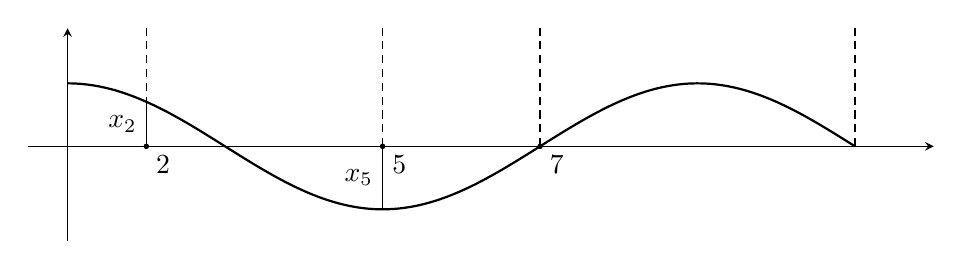
\begin{tikzpicture}[>=stealth, scale=1.0,samples=200]
  \draw [->](-0.5,0)--(11,0);
  \draw [->](0,-1.2)--(0,1.5);
  \draw [thick, domain=0:10]  plot (\x,{0.8*cos(0.25*pi*\x r)});
  \foreach \x in {2,5,7} 
    { \fill(\x-1,0)circle(1pt)node[below right]{\x}; }
  \draw[thin](1,0)--(1,{0.8*cos(0.25*pi r)})node[midway,left]{$x_2$};
  \draw[thin](4,0)--(4,{0.8*cos(pi r)})node[midway,left]{$x_5$};
  \foreach \x in {1,4,6,10 }{ \draw[thin,densely dashed] (\x,0)--(\x,1.5);}
\end{tikzpicture}
\end{document}